\section{Results}
\label{sec:results}
\begin{figure*}[t]
\centering
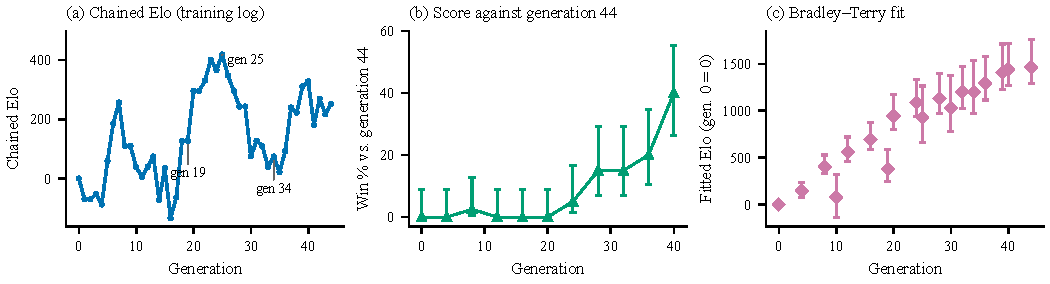
\includegraphics[width=\textwidth]{figures/elo_comparison.pdf}
\caption{Chained Elo says training stalled after generation~\valChainedPeakGen{}; anchored games say it kept
improving. (a)~Chained Elo from the training log (\valEvalGames{}-game matches against the previous
generation, \valEvalSims{} simulations). (b)~Score of every fourth generation against the final generation
\valNGens{} (\valEvalGames{} games each, \valAnchoredSims{} simulations), with 95\% Wilson intervals.
(c)~Bradley--Terry ratings fitted to all \valHtoHGames{} head-to-head games, with 95\% bootstrap intervals.
The model fits poorly at large rating gaps (see text), so read (c) as a ranking, not a scale.}
\label{fig:elo}
\end{figure*}

\paragraph{Chained Elo misranks the run.}
Figure~\ref{fig:elo}a shows the training log's chained Elo: a peak of \valChainedPeak{} at
generation~\valChainedPeakGen{}, a decline to \valChainedThirtyFour{} at generation~34, and \valChainedFinal{}
at the end. Every anchored measurement disagrees.
\begin{itemize}
  \item Head to head, generation~34 beats generation~25 in \valHTtfVsTf{} games and generation~19 in
        \valHTtfVsNt{}, and generation~\valNGens{} beats generation~34 in \valHFfVsTtf{}.
  \item Against the final generation, the scores of generations $0,4,\dots,40$ are \valAnchorScores{} wins
        out of \valEvalGames{}: flat at zero while the earlier networks are far weaker, then rising steadily
        from generation~24 (Figure~\ref{fig:elo}b), with no sign of the decline after generation~25.
  \item The Bradley--Terry ratings increase with generation apart from two less-constrained points (generations
        10 and 19, which appear only in a few long-range matches) (Figure~\ref{fig:elo}c).
\end{itemize}
The fit is approximate. Its Pearson $\chi^2$ is \valBTChiSq{} over \valBTMatches{} matches with
\valBTFree{} free ratings. Its residuals are systematic: in close pairs the newer network wins more often
than predicted, and in very lopsided pairs the weaker network still wins a few games, mostly through the
randomized opening. We therefore do not quote a total Elo gain from the fit.

\begin{figure}[t]
\centering
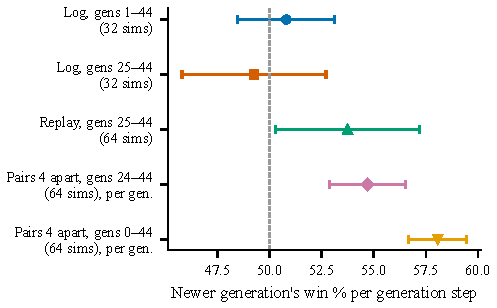
\includegraphics[width=\columnwidth]{figures/step_gain.pdf}
\caption{At 64 simulations, consecutive-generation matches agree with pairs four apart; the training log's
32-simulation matches measured almost no gain. Each row is the newer network's win rate for a single
generation step, with 95\% Wilson intervals; results for pairs four apart are converted to a single step
through the Elo scale. Compare rows over the same generations: gains are larger early in training.}
\label{fig:step}
\end{figure}

\paragraph{Why: noise contributes, but the cheap matches are the main cause.}
Pairs four generations apart give the newer network a pooled win rate of \valStepFourWr{}, or about
\valStepElo{} Elo per generation over the whole run. Over generations 24--44 alone, the rate is \valLateStepElo{}
Elo per generation, a per-generation win rate of \valLateStepWr{} (95\% interval \valLateStepWrLo{}--\valLateStepWrHi{}).
At that rate, chained Elo should have risen by about \valDropExpect{} from generation~25 to~34, with a
noise standard deviation of $3\times\valStepSE{}$ Elo. Instead it fell by \valInversion{}, \valDropZ{} standard
deviations from the expectation, so noise alone is an unlikely explanation.

The training log's matches were cheaper than our anchored ones: 32 simulations a move instead of 64.
Replaying the consecutive pairs from generation~\valConsFrom{} onwards at 64 simulations gives the newer network
\valConsWr{} of the games (95\% interval \valConsWrLo{}--\valConsWrHi{}), against \valConsWrLog{} for the same pairs
in the log. That is consistent with the \valLateStepWr{} implied by pairs four apart over the same generations
(Figure~\ref{fig:step}). Chained over generations 25 to 34, the replay gives \valReplayChain{} Elo, the correct direction
(the head-to-head result implies \valHtoHEloTtfTf{}), where the log gave $-$\valInversion{}. Over generations
\valConsFrom{}--\valNGens{} it gives \valReplayChainAll{}, where the log gave \valLogChainAll{}.

So comparing adjacent generations is not misleading in itself. In this run the per-generation matches were
too shallow to separate networks that, at deployment-like search depth, differ by a few dozen Elo, and summing
their noisy, compressed differences hid the trend. On any one pair the difference between the log and the
replay is within noise, so we cannot fully separate the effect of search depth from the play of chance with
one run. But every 64-simulation measurement in Figure~\ref{fig:step} points the same way.

\paragraph{External calibration.}
\label{sec:gnugo}
Against GNU~Go~3.8 at level \valGnuLevel{} (its weakest), with Chinese rules, komi 7.5 and
\texttt{-{}-capture-all-dead} so that our area scoring is fair to it, generation~\valNGens{} at \valGnuSims{}
simulations a move won \valGnuWins{} games, with a median losing margin of \valGnuMedianMargin{} points.
GNU~Go's own scoring named the same winner in \valGnuScoreAgree{} games. The internal gains above are real,
but in absolute terms the network remains far weaker than a classical engine at its weakest setting.

\paragraph{One engine, three runtimes.}
The rules are implemented three times: in Python for training, in Swift for the macOS app and in JavaScript
for the browser. All three agree exactly on the board, ko point, legal moves, score and input planes for
\valRuleCases{} positions taken from \valRuleGames{} random games, generated by the Python rules. The trained
network, exported to Core ML and to ONNX, matches PyTorch to within $\valCoreMLDiff\times10^{-6}$ and
$\valOnnxDiff\times10^{-6}$ on random inputs. On \valBenchPositions{} positions from a self-play game,
searched from scratch for \valBenchSims{} simulations each, the root visit counts were identical in
\valBenchIdentical{} positions on all three runtimes (Table~\ref{tab:platform}), so the app and the web page
make exactly the moves the trainer would.

\begin{table}[t]
\centering
\small
% generated by figures_scripts/platform_table.py
\begin{tabular}{@{}lrrrr@{}}
\toprule
Runtime & ms & sims/s & Same & Max $|\Delta|$ \\
\midrule
PyTorch & 974 & 411 & 15/15 & -- \\
Core ML & \textbf{534} & \textbf{750} & 15/15 & $5.5\times10^{-6}$ \\
ONNX (web) & 975 & 410 & 15/15 & $7.6\times10^{-6}$ \\
\bottomrule
\end{tabular}

\caption{The same search on three runtimes: PyTorch (Python trainer), Core ML (Swift app) and ONNX Runtime
Web (browser, WebAssembly). Columns: median time (ms) for a \valBenchSims{}-simulation search over
\valBenchPositions{} positions (best of three runs each, one leaf per network call, one CPU thread); positions
whose root visit counts equal PyTorch's exactly; largest network output difference from PyTorch.}
\label{tab:platform}
\end{table}
